\section{The Attribute-Trie Model}
\label{sec:model}

This section formalizes the organization introduced in~\cite{kapoor2020efficient}, which all later extensions preserve.

\subsection{Records, Tries, and Interval Labels}

\begin{definition}[Store and attribute trie]
A \emph{store} has an ordered schema $A=(a_1,\dots,a_m)$ and a multiset of records $D$, where record $r$ assigns a normalized value $r[a_\ell]$ to each attribute. The \emph{attribute trie} $T(D)$ is the smallest rooted tree in which every record $r$ is spelled by a root-to-leaf path $\langle \rho, v_1,\dots,v_m\rangle$ with $\mathrm{val}(v_\ell)=r[a_\ell]$, and siblings carry distinct values. Node $v_\ell$ is at level $\lev(v_\ell)=\ell$.
\end{definition}

Level $\ell$ therefore stores each distinct value of $a_\ell$ once per distinct prefix $(r[a_1],\dots,r[a_{\ell-1}])$. Records that share a prefix share its nodes. This prefix sharing is the source of the deduplication discussed in~\cite{kapoor2020efficient}. Records that agree on every attribute collapse into one path. Kiara presents such records once, so applications that need multiset semantics include a distinguishing attribute.

After loading, one depth-first traversal assigns each node two numbers from a single counter $c$. The counter is incremented when the traversal enters a node and again when it leaves it:
\begin{equation}
\pre(v) = c_{\mathrm{enter}}(v), \qquad \post(v) = c_{\mathrm{leave}}(v).
\end{equation}
Fig.~\ref{fig:trie} shows an example.

\begin{figure}[t]
\centering
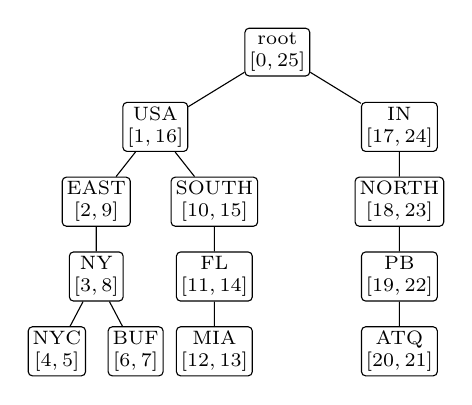
\begin{tikzpicture}[
  level distance=9.5mm,
  every node/.style={draw, rounded corners=1.5pt, font=\scriptsize, inner sep=1.6pt, align=center, fill=white},
  level 1/.style={sibling distance=31mm},
  level 2/.style={sibling distance=15mm},
  level 3/.style={sibling distance=11mm},
  level 4/.style={sibling distance=10mm},
  edge from parent/.style={draw, -}]
\node {root\\$[0,25]$}
  child {node {USA\\$[1,16]$}
    child {node {EAST\\$[2,9]$}
      child {node {NY\\$[3,8]$}
        child {node {NYC\\$[4,5]$}}
        child {node {BUF\\$[6,7]$}}}}
    child {node {SOUTH\\$[10,15]$}
      child {node {FL\\$[11,14]$}
        child {node {MIA\\$[12,13]$}}}}}
  child {node {IN\\$[17,24]$}
    child {node {NORTH\\$[18,23]$}
      child {node {PB\\$[19,22]$}
        child {node {ATQ\\$[20,21]$}}}}};
\end{tikzpicture}
\caption{Attribute trie for four records with schema (Country, Region, State, City). Each node is labeled with $[\pre,\post]$. The level-2 posting list for \texttt{EAST} is $\langle[2,9]\rangle$ and the level-4 list for every city holds one node. The query Region$=$EAST $\wedge$ City$=$BUF reduces to testing whether $[6,7]\subset[2,9]$.}
\label{fig:trie}
\end{figure}

\begin{lemma}[Ancestry as containment]
\label{lem:ancestry}
Node $u$ is a proper ancestor of $v$ if and only if $\pre(u)<\pre(v)$ and $\post(v)<\post(u)$.
\end{lemma}
\begin{IEEEproof}
This is the parenthesis property of depth-first search~\cite{cormen2009introduction}. The traversal enters $v$ after entering $u$ and leaves $v$ before leaving $u$ exactly when $v$ lies in the subtree of $u$.
\end{IEEEproof}

\begin{lemma}[Order within a level]
\label{lem:levelorder}
The intervals of distinct nodes at the same level are disjoint. Hence, ordering same-level nodes by $\pre$ is the same as ordering them by $\post$. Moreover, for any node $u$ with $\lev(u)<\ell$, the level-$\ell$ descendants of $u$ form a contiguous run in the $\pre$-ordered sequence of level-$\ell$ nodes.
\end{lemma}
\begin{IEEEproof}
Two same-level nodes are not ancestors of each other, so by the parenthesis property their intervals are disjoint, and disjoint intervals are ordered identically by either endpoint. The descendants of $u$ are exactly the nodes whose intervals lie inside $[\pre(u),\post(u)]$. Among pairwise disjoint intervals sorted by left endpoint, these occupy a contiguous range.
\end{IEEEproof}

\subsection{Level Indexes}
For each searchable level $\ell$, a hash index $I_\ell$ maps every key $k$ to a posting list $P_\ell(k)$ of level-$\ell$ nodes whose value yields key $k$. Kiara appends a node to its lists when the traversal \emph{leaves} the node. By Lemma~\ref{lem:levelorder}, every posting list is therefore sorted by $\pre$ without an explicit sort. This is the property that makes binary-search reduction possible~\cite{kapoor2020efficient}. In the 2020 design each node contributed one key. Section~\ref{sec:system} relaxes this so that a node contributes one key per element of a collection value, and adds ordered and interval structures over the key space of a level.

\subsection{Conjunctive Queries and Level-Wise Reduction}
A query $Q$ is a set of predicates, each constraining one attribute. For a constrained level $\ell$, let $C_\ell$ be the set of level-$\ell$ nodes whose values satisfy every predicate on $a_\ell$. Let $\ell_1<\dots<\ell_t$ be the constrained levels, and define
\begin{align}
R_1 &= C_{\ell_1}, \nonumber\\
R_i &= \{\, v\in C_{\ell_i} \;:\; \exists\, u\in R_{i-1},\ u \text{ is an ancestor of } v \,\}. \label{eq:reduction}
\end{align}

\begin{theorem}[Correctness of reduction]
\label{thm:reduction}
A record satisfies $Q$ if and only if its path passes through a node of $R_t$. The answer to $Q$ is the set of records spelled by root-to-leaf paths through $R_t$.
\end{theorem}
\begin{IEEEproof}
By induction on $i$, node $v$ at level $\ell_i$ belongs to $R_i$ exactly when the path from the root to $v$ passes through a node of $C_{\ell_j}$ for every $j\le i$. The base case is the definition of $R_1$. For the inductive step, each node has exactly one ancestor at level $\ell_{i-1}$, so the existential condition in~\eqref{eq:reduction} tests that unique ancestor. A record's path passes through its own value at every level. Therefore the record satisfies all predicates if and only if its node at level $\ell_t$ lies in $R_t$.
\end{IEEEproof}

Theorem~\ref{thm:reduction} holds for \emph{any} subset of constrained attributes. Once $R_t$ is known, its records are produced by walking parent pointers upward for attributes above $\ell_t$ and enumerating the subtree below each node of $R_t$ for attributes below it. By Lemma~\ref{lem:ancestry}, each ancestor test in~\eqref{eq:reduction} costs two integer comparisons. By Lemma~\ref{lem:levelorder}, a search over a sorted list either finds the unique candidate ancestor or delimits the contiguous run of candidate descendants.

\subsection{How Many Composite Indexes Would Be Needed?}
\label{sec:indexcount}

The motivation for the model is the number of composite indexes it avoids. We say a composite B-tree with key order $\pi=(\pi_1,\dots,\pi_k)$ \emph{serves} an attribute set $S$ by a full prefix seek if $S=\{\pi_1,\dots,\pi_{|S|}\}$.

\begin{proposition}
\label{prop:indexcount}
The minimum number of key orders that serve every nonempty $S\subseteq A$ by a full prefix seek is $\binom{m}{\lfloor m/2\rfloor}$.
\end{proposition}
\begin{IEEEproof}
The prefix sets of a key order form a chain in the Boolean lattice $2^A$. Serving every subset therefore requires a family of chains that covers the lattice. The subsets of size $\lfloor m/2\rfloor$ form an antichain of size $\binom{m}{\lfloor m/2\rfloor}$, and no chain contains two of them, which gives the lower bound~\cite{sperner1928satz,dilworth1950decomposition}. For the upper bound, the lattice admits a symmetric chain decomposition into exactly $\binom{m}{\lfloor m/2\rfloor}$ saturated chains $T_0\subset T_1\subset\dots\subset T_r$ with $|T_{i+1}\setminus T_i|=1$~\cite{debruijn1951set}. Each chain is realized by one key order that lists the elements of $T_0$ in any order, followed by the element added at each step. Every set in the chain is then a prefix set of that order.
\end{IEEEproof}

Table~\ref{tab:indexcount} compares this bound with the $2^m-1$ hash indexes needed for exact-match lookups on every subset and with the $m$ level indexes of the attribute trie. The 2020 article~\cite{kapoor2020efficient} reported $1+\sum_{k=1}^{m-1}k$ B-tree indexes, for example 46 for $m=10$. By Proposition~\ref{prop:indexcount} that count is below the lower bound of 252, so it cannot suffice. The corrected bound strengthens the original motivation. In practice, optimizers relax full prefix seeks into partial seeks plus residual filters, or intersect single-attribute indexes. Kiara is a structured instance of the latter approach, and Section~\ref{sec:results} measures it against both families.

\begin{table}[t]
\centering
\caption{Indexes Required to Serve Every Equality Conjunction Over $m$ Attributes}
\label{tab:indexcount}
\setlength{\tabcolsep}{4pt}
\begin{tabular}{@{}rrrr@{}}
\toprule
$m$ & Hash, $2^m-1$ & B-tree orders, $\binom{m}{\lfloor m/2\rfloor}$ & Attribute trie, $m$ \\
\midrule
5  & 31 & 10 & 5 \\
10 & 1{,}023 & 252 & 10 \\
20 & 1{,}048{,}575 & 184{,}756 & 20 \\
30 & $1.07\times10^{9}$ & $1.55\times10^{8}$ & 30 \\
50 & $1.13\times10^{15}$ & $1.26\times10^{14}$ & 50 \\
\bottomrule
\end{tabular}
\end{table}
